\documentclass[../main.tex]{subfiles}
\graphicspath{{\subfix{../IMAGES/}}}

\begin{document}
\localtableofcontents

\subsection{Basics of PV}

1 metric ton of coal cost around 100-120$\$/t$ (or 1.2cts/kWh of thermal energy). $1m^3$ of gas at home costs around 15cts/kWh of heat (1.5CHF/$m^3$). 1 litre of gasoline costs around 1.6CHF/l (or 17cts/kWh thermal and 56cts/kWh for mechanical energy). 1kWh of electricity at home is around 25-40cts/kWh.\\

World production of energy is 29470 TWh in 2023 with an annual growth of $2.6\%$. \\

 The mean solar irradiance is $1366 W/m^2$ in outer space. The spectrum is referred to as $AM_0$. On earth, we have losses by absorption and diffusion (Rayleigh scattering : blue light is more scattered than red light) : $1000W/m^2$.\\
 GHI : Global Horizon Irradiation (light arriving from all angles on an horizontal plane) up to $2700 kWh/m^2$.\\
 DNI : Direct Normal Irradiation (energy collected from the straight rays of the sun by a surface perpendicular to the rays; tracking the position of the sun) : up to $3650 kWh/m^2$.\\

 One year in Switzerland is equivalent to $1000-1500$ full hours at intensity $1000W/m^2$.\\

 \begin{theorem}
     \textbf{AMx} or Air Mass, where x describes the attenuation through the atmosphere : $x = \frac{1}{\cos \alpha}$. $\alpha$ the angle between the sun beam and the vertical direction. \textbf{AM0 :} solar spectrum outside of the atmosphere. \textbf{AM1 :} solar spectrum on earth when the sun is vertically above. \textbf{AM1.5 :} $1000W/m^2$, $\alpha = 48.19^\circ$. \textbf{AM1.5D :} only direct radiation ($900W/m^2$). \textbf{AM1.5G :} includes diffuse radiation ($1000W/m^2$).
 \end{theorem}

 \textbf{Ideal solar cells :} a photon absorber (a semiconductor with a bandgap) with two membranes : one to extract electrons and another one to extract holes. 

 \begin{figure}[hbt!]
     \centering
     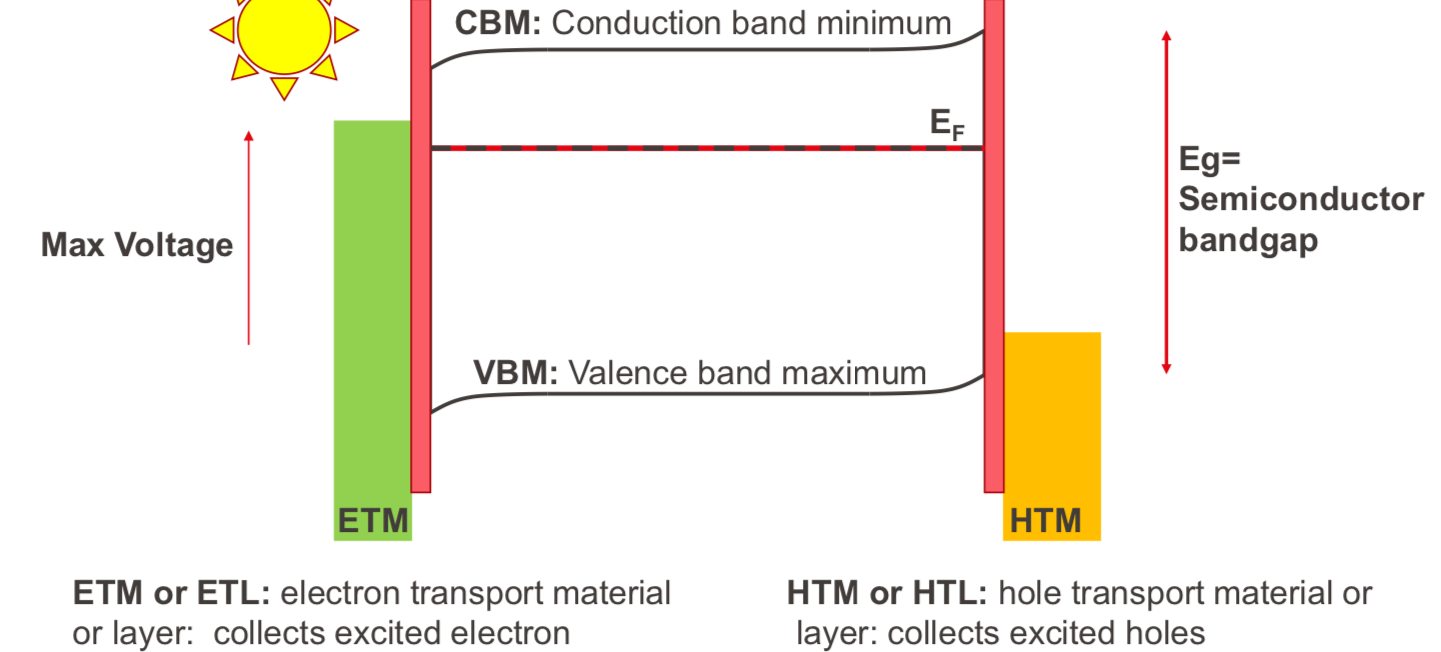
\includegraphics[width=0.7\linewidth]{IMAGES/PV/Screenshot 2025-02-18 at 14.25.18.jpeg.png}
 \end{figure}

 \quad \underline{Basic design :}\\
 Intrinsic (pure) semiconductor material. Doping with chosen impurities (becomes conductor with +(p) or -(n) charges transporting the current). Under light : absorption of photons if $h\nu > E_g$ (semiconductor bandgap). Photons absorbed in p-zone transfer their energy to electrons. \\

 Voltage depends on bandgap : $0.7V$ for crystalline Si, $1.1V$ for GaAs.\\
 Current depends on $E_g$ and is proportional to the surface area : typical $40 mA/cm^2$ c-Si.\\

 First approximation : a solar cell is a p-n diode with current source in parallel : \begin{equation}
     \begin{gathered}
         \text{Dark : } I_D = I_0 [e^{\frac{qV}{kT}}-1]\\
         \text{Illuminated : } I_L = I_D - I_{ph} = I_0 [e^{\frac{qV}{kT}}-1]-I_{ph}
     \end{gathered}
 \end{equation}

Then we have some parameters : $I_{sc}$ short circuit current, $V_{oc}$ open circuit voltage, $R_{MPP} = \frac{V_{MPP}}{I_{MPP}}$ the ideal power dissipation.\\
\textbf{Fill Factor :} $FF = \frac{P_{MPP}}{I_{sc} V_{oc}} = \frac{v_{oc}-\ln(v_{oc} + 0.72)}{v_{oc}+1}$, ($v_{oc} = \frac{V_{oc}}{k_BT/q}$); it indicates how square the I-V curve is. \\

Power/efficiency of a cell or module under defined STC : cell at $25^\circ C$, spectrum $AM1.5G$ and ght intensity at $1000W/m^2$. Efficiency at STC : $\eta_{STC} = \frac{P_{MPP}}{P_{light}}\rvert_{STC}$. Nominal power : $Wp = \eta_{STC} A$ (watt peak output).\\

With no bypass diode, likely working point is all cells at $V_{oc}$ and no current; no power out, no danger for the module. Or that all the voltage provided by the other cells applies in reverse onto shaded cells (breakdown and local heating).\\

Entrance voltage of an inverter can be up to $1000V$. Typical efficiency : $96/99\%$.\\

\begin{itemize}
    \item Wafer based (bulk semiconductor) : processing of wafers (100-400 microns), series connection
    \item Thin films : deposition of thin cells (micron) on large area substrate, monolithic series integration of the cells for high $V_{oc}$ and low $I_{sc}$.
\end{itemize}

\begin{figure}[hbt!]
    \centering
    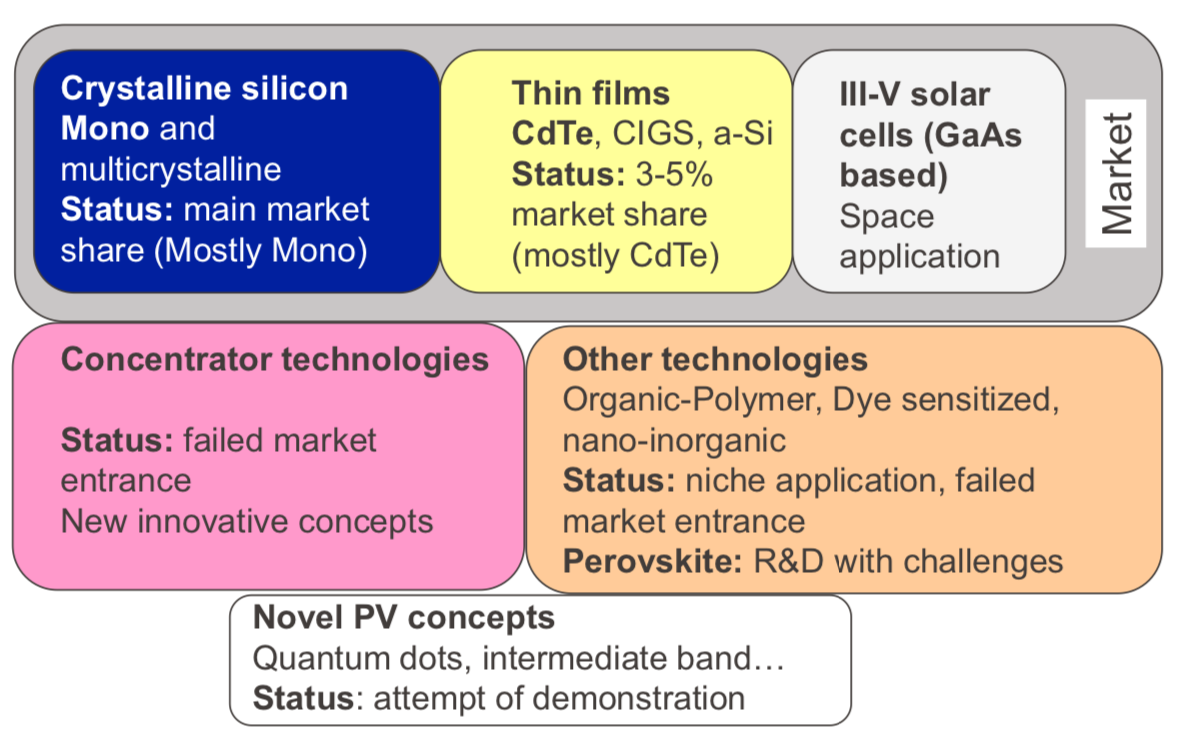
\includegraphics[width=0.6\linewidth]{IMAGES/PV/Screenshot 2025-02-18 at 14.56.30.jpeg.png}
    \caption{PV technologies}
\end{figure}

Semiconductor with a bandgap $E_g$ absorbs only photons with $E>E_g$. \begin{equation}
    \lambda [nm] = \frac{1240}{E(\lambda)[eV]}
\end{equation}

Single junction \textbf{Shockley-Queisser radiative limit} : radiative equilibium of cell under $AM1.5$ or one sun for a single junction. Ideal bandgap around 1.1 to 1.5$eV$. Limit of $31-33\%$.\\

With two junctions, Shockley-Queisser radiative limit is around $42\%$, with 3 it is around $49\%$, with infinity it is around $68\%$. Also, by increasing light intensity, we increase $V_{oc}$. Better use of the photon energy! $V_{oc} \simeq \frac{kT}{q} \ln (\frac{I_{sc}}{I_0}+1)$.\\

\textbf{Spectral response SR($\lambda$) :} the current in sc conditions per incident power as function of wavelength. $I_{cell, spec}= A \int_{300}^{1200}Spec(\lambda) SR(\lambda)d\lambda$.\\
\textbf{External Quantum Efficiency (EQE) : } ratio of collected electrons per incident photons at sc. $EQE(\lambda) = \frac{[electrons]}{[photons]}\rvert_{Isc} = SR(\lambda) \frac{E(\lambda)}{q}$. Want it to be close to 1.\\
\textbf{Internal Quantum Efficiency (IQE) : } $IQE(\lambda) = \frac{EQE(\lambda)}{1-R(\lambda)}$.

\warning PV are typically 30-100x more efficient than biomass per $m^2$.\\

\subsection{Technology, market and scenarios}
\begin{itemize}
    \item Crystalline Si : multi/mono $20-24\%$
    \item Thin film : $6$(a-Si)-$19.3\%$(CdTe)
    \item III-V and concentration : $25-35\%$
\end{itemize}

Annual module production : $500GW$ in 2023 ($13GW$ of thin-film, $4GW$ of multi-Si and $485GW$ of mono-Si) compared to $250MW$ in 2000.\\

III-V solar cells for space : market of 1MW, triple junction, high cell cost ($200$€/W), small volume, complex growth process.\\

Concentration light system : utilization of a smaller active cell area. If no series resistance is present in a solar cell, the $V_{oc}$ and FF increases. Maximum concentration of $45000$ (limited by the sun's size). \\


The initial disadvantage of crystalline silicon are the many steps needed.\\
Types of crystalline technologies : Al-BSF (aluminium backsurface field), PERC (passivated emitter and rear contact), TOPCON (tunneling oxide contact), SHJ (HJT, silicon heterojunction), IBC (interdigitated back-contacted solar cell).\\

Efficiency increase : more bubars (gain of $1\%$), half-cells (gain of $2\%$), larger cells (gain of $1\%$), larger modules (gain of $2\%$).\\

In 2023, the cumulative installed PV capacity was $1400GW$.\\

\textbf{LCOE (Levelised Cost of Electricity) :} $LCOE = \frac{CAPEX + total\: OPEX}{total\: electricity\: production}$ (CAPEX : capital expenditure, OPEX : operational expenditure). Around $10cts/W$ in 2024 for c-Si modules.\\
If you can use/sell at this price, you make your return on investment as planned. \\

Typical investment (CAPEX) is around 1€/W for midsize system, around 0.5-0.6€/W for large plants. \\
The direct LCOE costs of solar energy have become unbeatable in most countries in the world for new, large PP, down to 1.3-4cts/kWh possible (in CH it is around 10-20cts/kWh). This is 4times cheaper than a full new coal PP.\\

Objective : 1.5TW annual PV module production.\\
How much would it cost to put in place this production? $120M$€$/GW \Rightarrow 180$billions €.\\

In China : PV at $12cts/W$, battery cells at $50$€/kWh, windturbine at $40cts/W$, inverters at $3cts/W$, electrolysers at $30cts/W$.\\

Today automotive battery pack cost around $120$€/kWh.\\

\subsection{Energy yield and PV systems}
\subsubsection{Energy yields}

The energy yield is given in kWh produced/W installed. The nominal efficiency does not count for energy yield (can be the same for a 10 or 20$\%$ module). Typically, the AC injected power will be $70-90\%$ of the nominal power after correction. \\
Typical losses : heating effect ($3-15\%$ losses), lower irradiance ($1-3\%$), dust/soiling ($3-10\%$) module mismatch, connections cables, inverter/transformer losses ($2-10\%$), module degradation ($1\%$ at the beginning to $12-25\%$ after 30 years), others.\\

\warning For silicon and most semiconductor, $V_{oc}$ decreases while current increases a little with temperature : $-0.25 \%/\circ C$.\\
To quantify the thermal behavior of modules in typical op conditions : $800W/m^2$, $T_a = 20^\circ C$, free mounting, wind $1m/s$. \textbf{NOCT : }Nominal Operating Cell Temperature given in $V_{oc}$ conditions (around $45^\circ C$). \textbf{NMOT : }Nominal Module Operating Temperature T : module at MPP (in the range of $43^\circ C$).\\

Degradation : typically $0.4-0.5\%$ per year for c-Si ($0.7-1\%$ for thin film). With $2\%$ degradation the first year and $0.3-0.6\%$ per year afterwards. \\

To compare system performance independently from irradiation : \begin{equation}
    PR = \frac{\eta_{av}}{\eta_{STC}} = \frac{Y_f}{Y_r}
\end{equation}
With $\eta_{av}$ the average system efficiency, $\eta_{STC}$ the module STC efficiency, $Y_f$ the production yield in $kWh/kW_p$ and $Y_r$ the reference yield production (energy theoretically obtainable by kWp measured in kWh/kWp at nominal STC conditions).\\

\subsubsection{Bifacial PV and PV system}
The back is illuminated. Increases efficiency but import a lost of power ($2-3\%$ at STC). Ground reflection (Albedo) can add $5-30\%$ annual energy per Watt. PR can be larger than 1 but is system dependent. It can be combined with 1-axis tracking to gain $20-40\%$ energy.\\

Inverter types : Galvanically separated (no common ground, high level of security, contains transformer), not galvanically separated (common ground, more efficient, more complicated circuitry).\\

Battery connection can be in DC coupled configuration (higher efficiency, only one inverter, more compact) or in AC coupled configuration (battery can be added later). \\

\subsubsection{Applications}
\quad \underline{Building Integrated PV (BIPV) :} \\
A BIPV module is a PV module and a construction product together. A BIPV system is a photovoltaic system in which a PV modules satisfy the definition above.\\

It is possible to change the look of the cells : digital ceramic printing (printing on glass), interferial coatings, coloring foils...\\

\quad \underline{Floating PV :}\\
Use ponds, water reservoir. Currently at $1-1.2$€/W CAPEX. \\

\subsection{Sustainability of PV}
No limit in raw material supply : Silicon is the second most abundant material in earth crust. No rare elements in c-Si modules. They are recyclable. It uses $17g$ of silicon for $1g$ of module. A typical PV system will give back the energy required for fabrication in 1 year in CH. Full module require currently around $0.5-0.6kWh/Wp$. Modern processes of module fabrication : $10-20g CO_2/kWh$, for the full system : $20-35gCO_2/kWh$.\\

\subsection{Basic semiconductor properties}
\subsubsection{Intrinsic SC}

Energy bands : free electron (energy in 1D with wave factor k : $E = \frac{p^2}{2m} = \frac{(hk)^2}{2m}$), electron in a box of length L ($k_l = l \frac{2\pi}{L}$, $E = \frac{(h(\frac{2\pi }{L}l))^2}{2m}$, discrete k-states), periodic potential $V(x) = V(x+a)$ (Bloch theorem, periodicity in k with reciprocal lattice $G = \frac{2\pi}{a}$ : $E = \frac{h^2 (k+nG)^2}{2m}$), non-trivial periodic potential ($U = U_1(e^{ikx} + e^{-ikx})$, defined by Fourier component $U_1$).\\

Transitions between bands defines indirect(e.g. Si, Ge : weak absorption) and direct(e.g. GaAs : strong absorption) bandgaps. Transitions within a band is a charge transport, the curvature yields effective masses. 

\begin{figure}[hbt!]
    \centering
    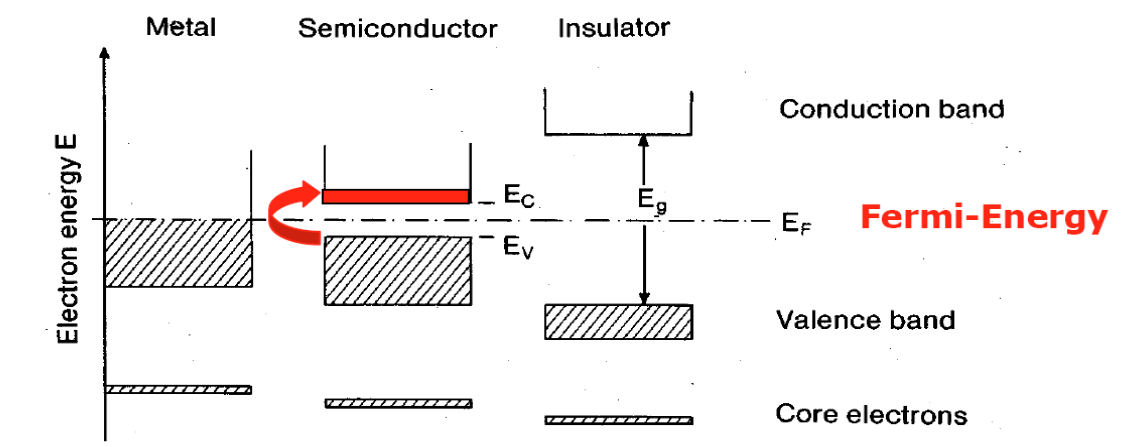
\includegraphics[width=0.7\linewidth]{IMAGES/PV/Screenshot from 2025-03-18 13-51-13.png}
\end{figure}

\begin{itemize}
    \item Metal : partially filled electronic band
    \item Semiconductor : a gap between bands, at $T=0K$ completely full band below gap and an empty above. At $T>0K$, electrons can jump across a small bandgap forming a hole below. Both types of carrier can transport current.
    \item Insulator : same as semiconductor, but large bandgap yields few thermally excited electrons and holes.
\end{itemize}


As electrons are fermions : Fermi-Dirac distribution function : \begin{equation}
    F(E,E_F)  = \frac{1}{1+\exp{(\frac{E-E_F}{kT})}}
\end{equation}
With $E_F$ the Fermi level. At $0K$, electrons fill the states up to the Fermi-level. $\mathbf{kT = 26meV}$ at $300K$.\\

The carrier denity is then (0 for thermal equilibrium) : $n_0 = n(E_F) = 2\int_{E>E_C} f_{FD}(E,E_F) d^3k = \int_{E_C}^\infty f_{FD}(E,E_F) g(E) dE$, with $g(E) = \frac{8\sqrt{2} \pi m_e^{*3/2}}{h^3} (E-E_c)^{1/2}$ (density of states).

If $E_F>3kT$ then approximate $f_{FD} \simeq f_{MB}$ and :
\begin{equation}
    \begin{gathered}
        n_0 = N_C\exp{\frac{E_F-E_C}{kT}}\\
        N_C = 2(\frac{2\pi m_e^*kT}{h^2})^{3/2}\\
        p_0 = N_V \exp(\frac{E_V-E_F}{kT})\\
        N_V = 2 (\frac{2\pi m_h^*kT}{h^2})^{3/2}\\
    \end{gathered}
\end{equation}

Effective density of states (electrons : $N_C$, holes : $N_V$). In intrinsic material : $n_0 = p_0$ thus $E_i = \frac{E_C + E_V}{2} + \frac{kT}{2} \ln \frac{N_V}{N_C}$ and also $p_0n_0 = N_CN_V \exp(\frac{-E_g}{kT}) = n_i^2$.\\
For example Si : $10^10 cm^{-3}$, Ge : $10^{13} cm^{-3}$, GaAs : $10^6 cm^{-3}$. $n_i$ increases exponentially with temperature. 

\warning $n_i^2$ plays an important role for the $V_{oc}$ as it relates $V_{oc}$ to the bandgap of the SC and governs the temperature dependence of $V_{oc}$.\\


\subsubsection{Extrinsic SC}

\quad \underline{Donors :} replace Si atom (group IV) in crystal lattice with group V element : extra electron

\quad \underline{Acceptors :} replace Si atom with group III element : extra hole\\

Electrons and holes can be treated like lowest orbit of the H atom but in different environment : electron mass is replaced by $m_e^*= 0.28m_e$, multiply vacuum permittivity $\varepsilon_0$ by relative permittivity of silicon ($\varepsilon_{Si} = 11.7$). The Bohr radius expands to $a_{Si} = 5-10nm$ (electrons and holes are delocalised over several atoms).

The binding energy is : $E_n = \frac{q^4 m^*}{2(4\pi \varepsilon_0 \varepsilon_{Si} h)^2} \frac{1}{n^2}$.\\

The densities of ionised donors and acceptors are now : \begin{equation}
    \begin{gathered}
        N_D^+ = N_D \frac{1}{1+2\exp(\frac{E_F-E_D}{kT})}\\
        N_A^- = N_A \frac{1}{1+4\exp(\frac{E_A-E_F}{kT})}\\
    \end{gathered}
\end{equation}

For homogeneous SC in darkness : $p_0 - n_0 - N_A^- + D_D^+ = 0$. For n-type material : $E_F-E_C = kT\ln \frac{n_0}{N_C}$ and for p-type : $E_V-E_F = kT\ln \frac{p_0}{N_V}$.\\

Extrinsic atoms can act as dopants but can also create other electronic levels : Trap states (capture carriers, thermally release them to same band), recombination centers (capture e- with h+ and recombine them). Some impurities can create multiple energy levels with a donor/acceptor character, can be coupled with recombination activity. Impurities which create deep levels (defects) usually yield poor material quality.\\


In a crystal, charge carriers move with random thermal velocity $<v_{th}> \simeq \sqrt{\frac{3kT}{m^*}} = 10^7 cm/s$ (at $T=300K$). Average time between 2 collisions (relaxation time) : $\tau_r = 10^{-13}s$. Mean free path : $l=v_{th} \tau_r = 10nm$, random motion on average $<x> = 0$.\\

With electric field $E$, carriers are accelerated for $\tau_r$ : $<v_{drift}> = a \tau_r$. Then, the electron/hole mobility : \begin{equation}
    \mu_e = \frac{\lvert <v_{drift} >\rvert}{\lvert E \rvert} = \frac{q \tau_r}{m_e^*},\: \mu_h = \frac{q\tau_r}{m_h^*}
\end{equation}


Random diffusion : carriers go to less populated regions $J_n^{diffusion} = qD_n \vec{\nabla} n$, $J_p^{diffusion} = -qD_p \vec{\nabla} p$, $D_n = \frac{kT}{q} \mu_n$ and $D_p = \frac{kT}{q} \mu_p$ are diffusion constant $[cm^2/s]$.\\

\subsubsection{Absorption and generation}
\begin{figure}[hbt!]
    \centering
    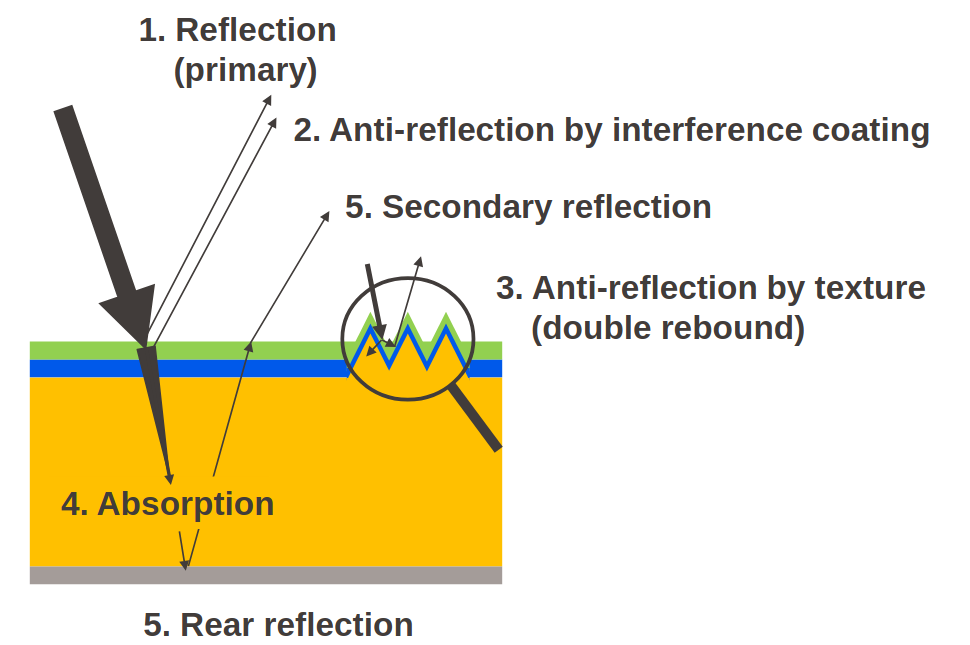
\includegraphics[width=0.5\linewidth]{IMAGES/PV/Screenshot from 2025-03-25 13-21-33.png}
\end{figure}

The \textbf{refractive index n} governs properties at interfaces. The \textbf{extinction coefficient $\kappa$} is the imaginary component of n. \\
Semiconductors are characterized by $n=3 \cdots 5$ in the visible region and $\kappa =0$ below $E_g$. \\
\textbf{Permittivity :} $\varepsilon = \varepsilon_1 + j \varepsilon_2 = (n+i\kappa)^2$ (or the dielectric function). Then : $n = \sqrt{\frac{\varepsilon_1 + \sqrt{\varepsilon_1^2+\varepsilon_2^2}}{2}}$, $\kappa = \sqrt{\frac{-\varepsilon_1 + \sqrt{\varepsilon_1^2+\varepsilon_2^2}}{2}}$.\\

The reflection at an interface : $R = \frac{(n_1-n_2)^2+\kappa_2^2}{(n_1+n_2)^2+\kappa_2^2}$. \warning Only valid for perpendicular incidence, $n_1$ is from transparent medium. For example : $n_{air}=1$, $n_{glass} = 1.5$, $n_{Si} = 4.1$, $\kappa_{glass} = 0$, $\kappa_{Si} = 0.03$.\\
For thin films, at each interface the wave is partially reflected and transmitted. Then : $r_{12} = \frac{n_1-n_2}{n_1+n_2}$. The phase is shifted by $180^\circ$ if it transmits from a high to low index material. We want that all waves reflected from the second interface and escaping the sample are at $180^\circ$ with the primary reflection : $\phi = 2\times 2 \pi n_2 \frac{d}{\lambda} = m\pi$ ($m$ an odd number). First AR reflection for :$n_2d = \frac{\lambda}{4}$.\\
In addition to the quarter wavelength conditions, zero reflection can be achieved for the minimum. The geometric mean is given by : $n_2 = \sqrt{n_1 n_3}$.\\

Reduction of reflection by texture : random pyramids (easy, double bouncing of the light, $R_{double} \simeq R_{single}^2$), inverted pyramids (requires masking), multiple bounces ($R_{tot} \simeq R^n \rightarrow 0$).\\
\begin{itemize}
    \item Indirect band gap SC : $\alpha_{ind} = (h\nu -E_g)^2$, in addition to the absorption of a photon, a phonon with energy $E_p$ must either be emitted/absorbed.
    \item Direct band gap SC : $\alpha_{dir} = \sqrt{h\nu-E_g}$.
\end{itemize}

In a semiconductor, the light intensity profile follows : $I(E,x) = I_0(E) e^{-\alpha(E) x}$, the \textbf{Beer-Lambert-Bouguer Law}. The $\kappa$ is the intensity decay of propagating waves : $\vec{E}(x,t) = \vec{E}_0 \exp(-\frac{2\pi \kappa}{\lambda} x) \exp(i(nk_0 x+\omega t))$. Then : \begin{equation}
    \alpha = \frac{4\pi \kappa}{\lambda} [cm^{-1}]
\end{equation}

The \textbf{spectral generation rate} is then : $G(\lambda,x) = \alpha \Phi_0(\lambda) e^{-\alpha(\lambda)x}$, $\Phi_0 [cm^{-2}nm^{-1}s^{-1}]$ the photon flux density entering at surface. Then : $G(x) = \int G(\lambda,x)d\lambda$.\\

\subsection{Generation/recombination}
Hot carriers interact with phonons on a time scale of the relaxation time $\tau_r$ (fs, ps). They arrive at the band edges where they can stay for the duration of the bulk lifetime $\tau_{bulk}$ ($\mu s$, ms). The process is called thermalization resulting in a steady state between supply of thermalizing carriers and recombination across the band gap. Under light/with carrier injection, steady state  with excess carrier density ($n = n_0 + \Delta n$, $p=p_0+\Delta p$ with $np>n_i^2$). \\
$\tau_{bulk}$ is the average time between generation and recombination of an e-h pair $\tau_n = \frac{\Delta n}{R}$, $\tau_p = \frac{\Delta p}{R}$.\\
Since $\tau_{bulk} >> \tau_r$, steady-state concentrations n and p are independent carrier population. \\
When no carriers are extracted : recombination rate R = optical generation rate G ($\Delta n = G\tau$). If dark : unique Fermi level. If illuminated : define independent quasi Fermi Levels (QFLs). \\

Lifetime measurement : apply known generation rate G, measure $\Delta n$ (through reflectivity of charge carrier plasma), determine $\tau$ (transient by exponential decay of $\Delta n$), assess recombination process.\\

For example, under $G=1$sun, we define the implied open circuit voltage : $iV_{oc} = \frac{E_{F,n} - E_{F,p}}{q} = \frac{E_c}{q} + kT \ln(\frac{n_0+\Delta n}{N_c}) - \frac{E_c}{q} + kT \ln(\frac{p_0+\Delta n}{N_v}) = kT \ln(\frac{(n_0+\Delta n)(p_0+\Delta n)}{n_i^2})$.\\

\textbf{Radiative recombination :}\\
Recombination of an electron and a hole : inverse process to absorption (always present), in direct SC : very effective, in indirect SC : needs phonon assistance. $R_e = R_{ec} np$ with $R_e$ the recombination rate and $R_{ec} [cm^{3} s^{-1}]$ the recombination coefficient. In ss with illumination, the net radiative recombination rate is given by : $R_{rad} = R_e - G_{th} = R_{ec} (pn-n_i^2)$.\\

For a n-type SC : \begin{equation}
    \begin{gathered}
        \text{Low-injection :}\: (n\simeq n_0, p\simeq \Delta p)\: R_{rad} = R_{ec} n_0 \Delta p = \frac{\Delta p}{\tau_p}\\
        \text{High-injection :}\: (n\simeq \Delta n, p\simeq \Delta p)\: R_{rad} =R_{ec} \Delta n \Delta p = \frac{\Delta p}{\tau_p}\\
    \end{gathered}
\end{equation}

The \textbf{Auger-Meitner recombination :} energy of recombination transferred to another charge carrier instead of a photon. Electron into high CB state, hole into low VB state : $R_{Aug} = C_nn^2p+C_p np^2$.\\
Auger processes are always relevant for high carrier densities, regardless whether doping or injection. \\

For a n-type SC : \begin{equation}
    \begin{gathered}
        \text{Low-injection :}\: (n\simeq n_0, p\simeq \Delta n)\: \tau_{p,Aug} = \frac{\Delta n}{R_{Aug}} = \frac{\Delta n}{C_n n_0^2 \Delta n + C_p n_0 \Delta n^2} \simeq \frac{1}{C_n n_0^2}\\
        \text{High-injection :}\: (n\simeq \Delta n, p\simeq \Delta n)\: \tau_{p,Aug} = \frac{\Delta p}{R_{Aug}} = \frac{\Delta p}{(C_n +C_p )\Delta n^3} \simeq \frac{1}{(C_n+C_p) \Delta n^2}\\
    \end{gathered}
\end{equation}

The \textbf{Schockley-Read-Hall recombination :} recombination via trapping levels close to midgap. Often the most important recombination process in solar cells. 
\begin{figure}[hbt!]
    \centering
    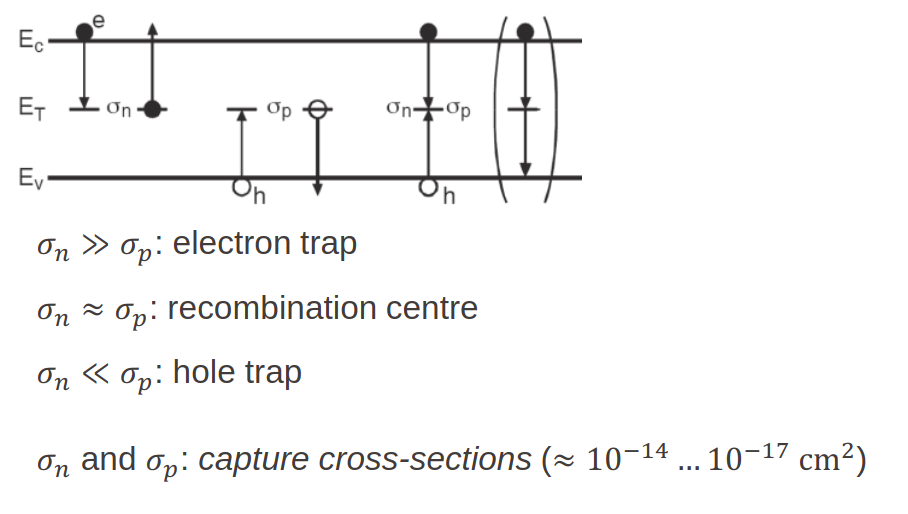
\includegraphics[width=0.5\linewidth]{IMAGES/PV/Screenshot from 2025-04-01 14-26-45.png}
\end{figure}
For defect states with density $N_t$ at an energy $E_t$ : $R_{SRH} = \frac{\nu_{th} N_t (np-n_i^2)}{\frac{1}{\sigma_p} (n+n_1) + \frac{1}{\sigma_n} (p+p_1)}$, with $n_1 = n_i e^{(E_t-E_F^i)/kT}$, $p_1 = n_i e^{-(E_t-E_F^i)/kT}$.\\

For a n-type SC : \begin{equation}
    \begin{gathered}
        \text{Low-injection :}\: (n\simeq n_0, p\simeq \Delta n)\: \tau_{SRH} = \frac{\Delta p}{R_{SRH}} = \frac{1+\frac{2n_i}{N_D} \cosh(\frac{E_t-E_i}{kT})}{\sigma \nu_{th} N_t} \simeq \frac{1}{C_n n_0^2}\\
        \text{High-injection :}\: (n\simeq \Delta n, p\simeq \Delta n)\: \tau_{p,0} = \frac{1}{\sigma_p \nu_{th} N_t}, \: \tau_{n,0} = \frac{1}{\sigma_n \nu_{th}N_t}, \: \tau_{p,n} = \tau_{p,0} + \tau_{n,0}\\
    \end{gathered}
\end{equation}

The total recombination rate is the sum of multiple processes : $\frac{1}{\tau_{bulk}} = \frac{1}{\tau_{rad}} + \frac{1}{\tau_{Auger}} + \frac{1}{\tau_{SRH}}$.\\


Photoluminescence imaging : radiative emission only visible when other recombination mechanisms are weak, bright areas in PL image is equivalent to good material. IR light source for uniform G and low pass filter in front of the camera to reflect laser.\\
Dark area indicate low lifetimes.\\
The rate of spontaneous emission is given by : $r_{em} = \alpha(h\omega) \frac{(nh\omega)^2}{\pi^2 h^3 c^2} \frac{1}{\exp(\frac{h\omega-\Delta E_F}{kT})-1}$.\\


\textbf{Wafer recombination :} wafer surface has some abrupt ending of crystal lattice that creates states within gap. The surface recombination rate is then : $R_s = S \Delta n_s$ with $S$ the surface recombination velocity (SRV). Then : $R_{S,SRH} = \frac{\nu_{th} D_{it} (n_sp_s-n_i^2)}{\frac{1}{\sigma_p} (n_s+n_1) + \frac{1}{\sigma_n} (p_s+p_1)}$, $D_{it} [cm^{-2}]$ the surface state density.\\
For low $\Delta n$, $n_s=n$, $p_s=p$, we get : $S_p = \sigma_p \nu_{th} D_{it}$.\\
The surface recombination current is defined by : $j_{surf} = q S_{eff} \Delta n(x=d) = qU_s(n,p)$ with $R_S = S_{eff} \Delta n(x=d)$.\\
Effective lifetime. Limiting cases : badly passivated surfaces ($\tau_{surf} = \frac{1}{D} (\frac{W}{\pi})^2$) and well passivated surfaces ($\tau_{surf} = \frac{W}{S_{front} + S_{rear}}$).\\

\subsection{Equations of solar cells}
Potential : $E = -\nabla \Phi$, Poisson equation : $\nabla \Phi = -\frac{\rho}{\varepsilon \varepsilon_0}$ and the charge density : $\rho = q(p-n+N_D^+ - N_A^-)$. \\

Depletion approximation : space charge region. Before contact : neutral regions and ionized dopants (one p region, one n region). After contact : electrons and holes recombine, SCR of ionized dopants. 
\begin{figure}[hbt!]
    \centering
    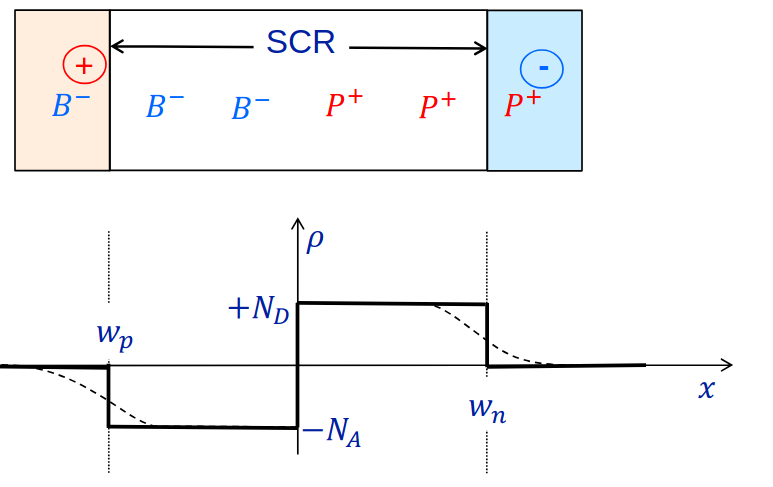
\includegraphics[width=0.5\linewidth]{IMAGES/PV/Screenshot from 2025-04-08 13-24-32.png}
\end{figure}

The charge neutrality is given by : $qN_A w_p = q N_D w_n$. The electrostatic potential is then : $\Phi=0$ at $x=w_p$ and $\Phi = V_{bi}$ at $x=w_n$. Parabolic variation. Electric field is linear.\\
The energy band diagram is such that : $E_{vac} = -q\Phi$. $qV_{bi} = kT \ln \frac{N_DN_A}{n_i^2}$.\\
If $V_{fwd}>0$ on the p-side : flatter output $q(V_{bi} - V_{fwd}$, generates a lot of current. If $V_{rev}<0$ on the p-side : steeper output $q(V_{bi} + \lvert V_{rev} \rvert )$, generates a small negative current.\\

\underline{How to calculate the $j(V)$ characteristic?} Assume : abrupt SCR and neutral SC beyond, carrier densities n and p linked to $\Phi$, low injection, no recombination and generation within the SCR. \\

Determine band bending with bias : $V_{bi} \pm V$, determine injection level at edge of SCR, solve drift-diffusion equation for neutral bulk, from solution for n and p assume pure drift current and determine $j_p$
 and $j_n$.\\
 \begin{itemize}
     \item Equilibrium carrier densities (dark, no-bias) : majority carrier densities need indices n and p to denote regions. $V_{bi} = \frac{kT}{q} \ln \frac{p_{p,0}}{p_{n,0}}$, with $p_{p,0} = N_A$ and $p_{n,0} = \frac{n_i^2}{N_D}$
     \item Injection at edges of SCR (dark, with bias) : with forward bias ($V<V_{bi}$), no longer in equilibrium but in ss. Majority in p-region : $p_{p,0}$ unchanged, minority in n-region : $p_{n,0} \rightarrow p_n$ modified : $p_n(w_n) = p_{n,0} \exp(\frac{qV}{kT})$.
     \item Carrier injection into quasi-neutral region : for holes in n-region : $\frac{\partial p_n}{\partial t} = G-R_p - \frac{1}{q} \nabla J_p = 0$, in dark ss 1D : $-\frac{1}{q} \frac{d j_p}{dx} = R_p = \frac{p_n-p_{n,0}}{\tau_p}$. Outside of SCR $j_p = -q D_p \frac{dp_n}{dx}$.\begin{equation}
         \begin{gathered}
             p_n(x) - p_{n,0} = p_{n,0} [\exp(\frac{qV}{kT})-1] \exp{-\frac{x-w_n}{L_p}}\\
             n_p(x) - n_{p,0} = n_{p,0} [\exp(\frac{qV}{kT})-1] \exp{\frac{x-w_p}{L_p}}\\
         \end{gathered}
     \end{equation}
     with $L_p = \sqrt{D_p \tau_p}$.
 \end{itemize}

 We know that : $j_{tot} = j_{maj} + j_{min}$. \\
 For an infinite cell : $j_{0,n} = \frac{qn_i^2}{N_D} \sqrt{\frac{D_p}{\tau_p}}$ and $j_{0,p} = \frac{q n_i^2}{N_A} \sqrt{ \frac{D_n}{\tau_n}}$.\\
 For high cell efficiency, $j_0$ should be low : small $n_i^2$, high lifetime, high doping. \\


 \underline{Illuminated cells :}\\
 For holes in n-region : $p_n(x) = (p_{n,0}[\exp(\frac{qV}{kT})-1]-G\tau)\exp\frac{w_p-x}{L_p} + G\tau_p + p_{n,0}$. Then : $j_p = j_{0,n} [\exp(\frac{qV}{kT})-1]-qGL_p$ (same for the p-side). Current from SCR : $j_{SCR} = qGw$. Photocurrent is then : $j_L = qG(L_n + L_p + w)$. Then : \begin{equation}
     j(V) = j_0 [\exp(\frac{qV}{kT})-1] - j_L
 \end{equation}

 Solar cells parameters are then : $j_{sc} = j_L$, $V_{oc} = \frac{kT}{q} \ln \frac{j_{sc}}{j_0}$, $FF = \frac{V_{MPP}}{V_{oc}} \frac{j_{MPP}}{j_{sc}}$, conversion efficiency : $\eta = \frac{FF\cdot V_{oc}\cdot j_{sc}}{P_{light}}$.\\

 Cell is not infinite : Geometry factor $G_F$ : $j_{0,p} = \frac{qn_i^2D_n}{N_A L_n} G_F$. Then : $j(V) = j_0 [\exp\frac{qV}{kT} -1]-j_L$, $j_{0,n} = \frac{qD_pn_i^2}{L_p N_D}G_{F,n}$ and $j_{0,p} = \frac{qD_nn_i^2}{L_n N_A}G_{F,p}$.\\

 \begin{figure}[hbt!]
     \centering
     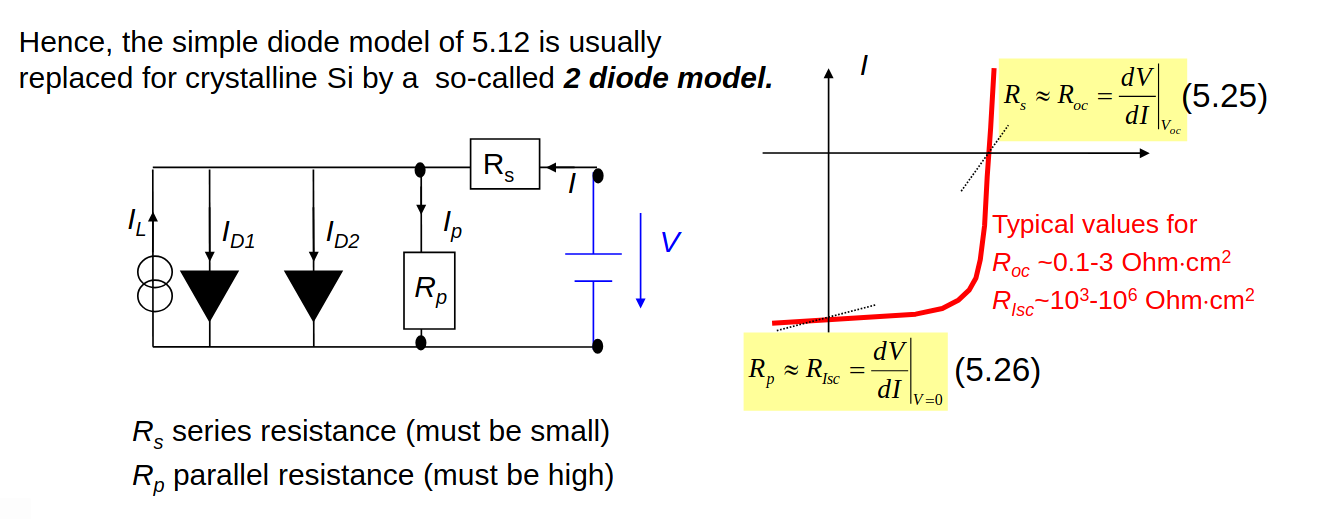
\includegraphics[width=0.5\linewidth]{IMAGES/PV/Screenshot from 2025-04-08 14-59-02.png}
 \end{figure}



\subsection{Silicon material and wafer preparation}
In 2024, a high quality mono-crystalline wafer costs 3cts/W to produce. \\
Preparation : 
\begin{itemize}
    \item Preparation of metallurgical grade (MG) Si : reduction of quartz sand with graphite in an arc furnace at high temperature ($SiO_2+2C \rightarrow Si+2CO$), requires around $14kWh/kg_{Si}$, around $1\%$ of impurities left.
    \item Purification via gas phase : Siemens process route with Tricholorosilane (TCS, Cleaning is performed by repeated distillation : $Si+3HCl \rightarrow SiHCl_3 + H_2$, uses around $40kWh/kg_{Si}$) or, fluidized bed reactor route with silane (avoids the need for cold walls) or, direct metallurgical silicon refinement.
    \item Fabrication of polycrystalline Si rods or granules
    \item Growth of single crystals with Czochralski or float-zone growth.
    \begin{figure}[hbt!]
        \centering
        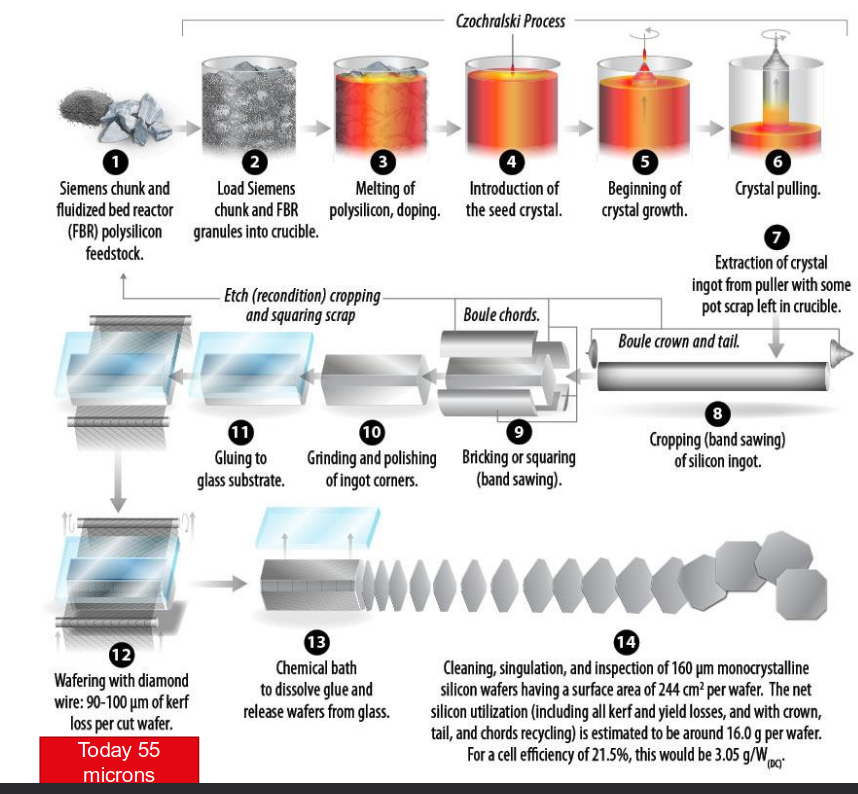
\includegraphics[width=0.5\linewidth]{IMAGES/PV/Screenshot from 2025-04-29 13-56-31.png}
    \end{figure}
    
    \item Cutting into wafers.
\end{itemize}
Chinese polysilicon price at 5€/kg in 2025. Outside at 19€/kg.\\
The goal is to have less than ppba (part per billion) dopants, and less than ppbw (ppb weight) of heavy metal impurities.\\

\begin{figure}[hbt!]
    \centering
    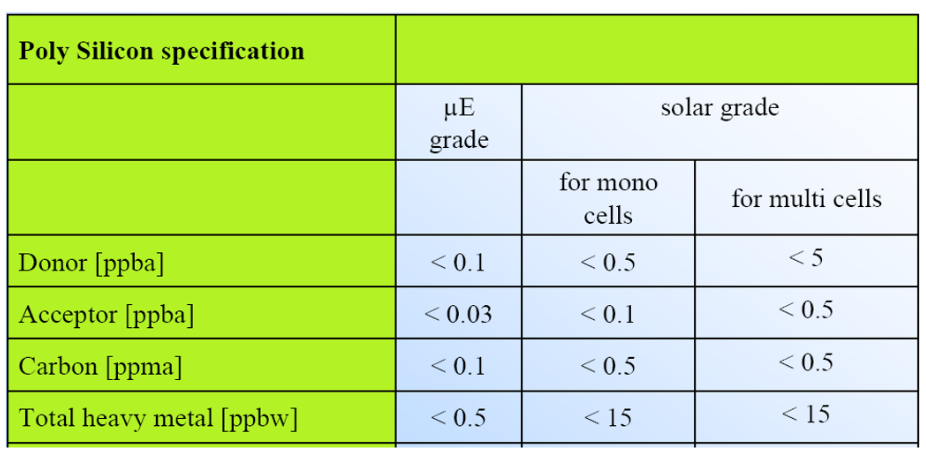
\includegraphics[width=0.5\linewidth]{IMAGES/PV/Screenshot from 2025-04-29 13-28-30.png}
\end{figure}
In 2025, typical wafer thicknesses : 150$\mu m$ PERC, 130$\mu m$ TOPCON, 110$\mu m$ Heterojunctions.\\
The better the passivation of surfaces, the thinner you can become. \\
Silicon is a hard, brittle material. Cracks make the wafers weak. To have stronger wagers, the cracks have to be smaller : this is why you need to etch wafers. For a semi-infinite plate : $\sigma_c = 0.82 (\pi a)^{-1/2} K_{IC}$, $K_{IC}$ the fracture toughness (for Si : $0.8-0.9MPa\: m^{1/2}$, GaAs : $0.31-0.46 MPa\: m^{1/2}$).\\

In the future, 1TW of PV per year will be equivalent to 2Mtons of Si per year. A modern monocrystalline module needs $0.4-0.5$ electrical kWh to produce in 2025.


\end{document}